\chapter*{Введение}							% Заголовок
\addcontentsline{toc}{chapter}{Введение}	% Добавляем его в оглавление
Диссертация подготовлена на кафедре высшей математики и исследования операций Института математики, механики и компьютерных наук им. И.И.\,Воровича Южного федерального университета и касается применения методов теории вязкостных решений в прикладных
задачах оптимального управления 

\textbf{Актуальность темы.}
Задачи оптимального управления естественным образом возникают в экономике, механике, экологии, менеджменте, финансовой математике и других областях. Динамические задачи оптимальной организации производства, эксплуатации природных ресурсов, назначения цен на товары, торговли рисковыми активами, распределения трудовых ресурсов и капитала, управления механическими системами и другие прикладные задачи требуют развития эффективных методов их решения. 

Основным общим подходом к анализу разнообразных задач оптимального управления является метод динамического программирования Беллмана. Данный метод зародился в 1960-х годах работах Р.\,Беллмана, но его применимость к непрерывным задачам оптимального управления долгое время представлялась весьма ограниченной в связи тем, что функция ценности (функция Беллмана), которая в каждой задаче формально удовлетворяет соответствующему уравнению Гамильтона-Якоби-Беллмана (HJB), часто является негладкой.
Ситуация изменилась в 1980-х годах в связи с изобретением и дальнейшим бурным развитием теории вязкостных решений: см., в частности, Crandall, Lions\cite{CraLio84}, Jensen\cite{Jen89}, Crandall, Ishii, Lions\cite{CraIshLio92}. Современное состояние теории вязкостных решений отражено в монографиях Fleming, Soner\cite{FleSon06}, Giga\cite{Giga06}, Pham\cite{Pha09} Touz\cite{Tou13}, [Koike], Katzourakis\cite{Katz14}. Данная теория не только позволила, в типичных ситуациях, описать функцию Беллмана как единственное вязкостное решение уравнения Гамильтона-Якоби-Беллмана, но и дала возможность развить новую схему обоснования сходимости численных методов для широкого класса сложных нелинейных задач: см. Barles, Souganidis\cite{BarSou91}, Oberman\cite{Obe06}. А именно, если для уравнения HJB справедлива теорема сравнения, то аппроксимирующая схема, обладающая свойствами монотонности, устойчивости и согласованности, является сходящейся.

Таким образом, возникла общая схема исследования широкого класса непрерывных  задач оптимального управления, предполагающая характеризацию функции Беллмана как единственного вязкостного решения уравнения HJB, доказательство теоремы сравнения, и построение монотонной, устойчивой и согласованной аппроксимирующей схемы. Данная схема является основой многочисленных современных исследований теоретического и прикладного характера. Отметим, несколько недавних работ, в которых рассматриваются конкретные прикладные задачи: торговля парами с нестационарной волатильностью Li, Tourin\cite{LiTour16}, вычисления цен безразличия неторгуемых активов на основе экспоненциальной полезности Henderson, Liang\cite{HenLian2016}, управлении запасами энергии при случайных ценах в условиях неполной информации Shardin, Sz{\"o}lgyenyi \cite{ShaSzo16}, оптимизации условной стоимостной меры риска (CVaR) в непрерывном времени Miller, Yang \cite{MilYan17}, оценивания и хеджирования контрактов на  энергетических рынках Callegaro\cite{Callegaro2017}, , управления диффузионными процессами со случайными дисконтирующими факторами, зависящими от фазовой переменной Lu, Yin, Guo, \cite{LuYinGuo17}, стратегий торговли в модели с байесовским обновлением параметра Baradel, Bouchard, Dang\cite{BarBouDan16}, загрязнения мелкого озера Kossioris, Loulakis, Souganidis\cite{KosLouSouPan17}, добычи нефти и ее налогообложения Pemy\cite{Pemy17}, инвестирования и выплаты дивидендов в модели с переключением режимов и налогообложением (Xu, Yao, Cheng, 2017), инвестирования-потребелния при наличии операционных издержек (Tsai, Fahim, 2018), оценки Европейских опционов в эксопненциальных моделях Леви с марковским модулированием (Momeya, 2018), управления процессом ирригации (Unami, Mohawesh, 2018) . 

Несколько известных задач, поддающихся анализу с использованием развитых в теории оптимального управления численных методов описаны в недавней обзорной работе работе Festa et. al. \cite{Festa17}: задача о восстановлении формы трехмерного объекта по закраске полутонового изображения (shape-from-shading), задача об управлении парусной лодкой, задача о распространении фронта, а также игры среднего поля (mean-field games). Отметим также обзор Neilan, Salgado, Zhang\cite{NeiSalZha17}, касающийся анализа численных схем для сильно нелинейных уравнений в частных производных на основе теории вязкостных решений. 

Развитие описанной методики представляется интересной и актуальной проблемой. Конкретные задачи, рассматриваемые в работе, представляют самостоятельный интерес и, в то же время, служат стимулом для развития и совершенствования данной методики. Они также позволяют лучше понять области ее применимости.

\textbf{Цель} настоящей работы состоит в исследовании конкретных прикладных задач оптимального управления на основе единой методики, основанной на теории вязкостных решений. Такая цель предполагает и развитие указанной методики, включающей (i) обоснование корректности описания функции ценности (функции Беллмана) как единственного вязкостного решения уравнения Гамильтона-Якоби-Беллмана, (ii) аналитическое исследование данного уравнения, (iii) построение и обоснование сходимости разностных схем на основе теоремы сравнения, (iv) проведение компьютерных экспериментов. В работе рассмотрены (1) задача об оптимизации потока дивидендов, перестрахования и инвестирования в диффузионной модели, (2) регулярная задача стохастического оптимального управления с конечным топливом, (3) задача об оптимальных стратегиях производства и назначения цены в динамической модели фирмы-монополиста, (4) задача о позиционировании случайного объекта за счет однократного изменения приращений его траектории. Основная цель при анализе каждой из этих задач состояла в описании структуры оптимального управления.

\textbf{Научная новизна.} (1) В задаче об оптимизации потока дивидендов страховой компании, которая использует стратегии перестрахования и инвестирования, с помощью численных экспериментов установлен ряд нетривиальных свойств оптимальных стратегий, касающихся зависимости барьерной структуры выплаты дивидендов, доли капитала, инвестируемой в рисковый актив, и стратегии перестрахования от случайного фактора, определяющего величину сноса рискового актива.
(2) В регулярной задаче стохастического оптимального управления с конечным топливом с использованием стохастического метода Перрона установлено, что функция Беллмана является единственным вязкостным решением задачи Дирихле для соответствующего уравнения Гамильтона-Якоби-Беллмана. На основе этого результата обоснована сходимость построенных разностных схем для задач оптимальной коррекции и оптимального слежения за стохастической системой с устойчивой или неустойчивой точкой равновесия. На основе численных экспериментов дано качественное и количественное описание оптимальных стратегий. 

(3) В задаче об оптимальных стратегиях производства и назначения цены в динамической модели фирмы-монополиста с использованием теории вязкостных решений и двойственности Фенхеля получено представление для функции Беллмана, исследована ее регулярность, и дано полное описание оптимальных стратегий без предположения о выпуклости оптимизационной задачи. Из полученных результатов следует, что невыпуклость функции производственных затрат способна объяснить наличие производственных циклов, но не накопление запасов. Проведен детальный анализ одной из функций затрат, рассматривавшейся Арваном и Мозесом \cite{ArvMos81} в 1981 году.

(4) В задаче о позиционировании случайного объекта за счет однократного изменения приращений его траектории, для моделей броуновского движения со сносом и геометрического броуновского движения, аналитически получены односторонние оценки области остановки. Точность данных оценок иллюстрируется численными экспериментами, в которых область остановки вычисляется исходя из решения методом конечных разностей уравнения Гамильтона-Якоби-Беллмана для соответствующей задачи оптимальной остановки. 

\textbf{Методы исследования.} В работе использованы методы теории оптимального управления диффузионными процессами, методы теории вязкостных решений уравнений Гамильтона-Якоби-Беллмана, методы выпуклого анализа, численные методы и компьютерные эксперименты. 

\textbf{Научная и практическая ценность работы.} Полученные результаты касаются качественного и количественного исследования ряда прикладных задач оптимального управления диффузионными и детерминированными процессами. С теоретической точки зрения представляет интерес развитие методики анализа таких задач (на математическом уровне строгости) на основе теории вязкостных решений. Полученные результаты могут использоваться специалистами в соответствующих предметных областях и служить иллюстративном материалом в учебном процессе в рамках специальных курсов по оптимальному управлению. Практическая ценность рассматриваемой методики состоит в том, что она позволяет получать качественные и количественные результаты о структуре оптимального управления на основе компьютерных экспериментов.

\textbf{Апробация работы.} Результаты, относящиеся к диссертации, излагались на следующих конференциях:
.....................................................

\textbf{Публикации.} Результаты работы опубликованы в 4 журнальных статьях в рецензируемых изданиях, входящих в базу данных Scopus (3 статьи) и в список ВАК (1 статья). Имеются также ... публикаций в тезисах международных конференций. 

\textbf{Личный вклад автора.} В работах, выполненных в соавторстве с научным руководителем, вклад авторов можно оценить как равный. В частности, компьютерная реализация разностных схем принадлежит соискателю. 

\textbf{Структура работы и объем диссертации.} Работа состоит из введения, четырех глав, заключения и библиографического списка. 

\textbf{Содержание работы.}
\textbf{В главе 1} рассматривается задача об оптимальной выплате дивидендов страховой компанией в диффузионном приближении.
Пусть имеется рисковый актив, цена которого $S$ описывается стохастическим дифференциальным уравнением
\begin{equation} \label{eq:1.1.2}
dS_t= \mu_2 (Y_t) S_t dt +\sigma_2 (Y_t) S_t d W^2_t.
\end{equation}
Здесь $Y$ случайный фактор, динамика которого подчиняется уравнению
\begin{equation} \label{eq:1.1.3}
dY_t=\mu_3(Y_t)dt+\sigma_3 (Y_t) d W_t^3.
\end{equation}
Стандартные броуновские движения $(W^1,W^2,W^3)$ предполагаются независимыми.

Модель резерва страховой компании заимствована из \cite{AsmHojTak00, HogTak04}:
\begin{equation} \label{eq:1.1.1}
d R_t=\mu_1(a) dt+\sigma_1 (a) dW^1_t,
\end{equation}
где $W^1$ --- стандартное броуновское движение.

Компания может инвестировать средства в данный актив, но объем этих инвестиций $\theta$ ограничен некоторой постоянной величиной $\overline\theta$. Пусть, кроме того, компания применяет динамическую стратегию $\alpha=(\alpha_t)_{t\ge 0}$ перестрахования и выплачивает дивиденды с конечной интенсивностью $c=(c_t)_{t\ge 0}$.
Приращение капитала $V$ компании складывается из приращений резерва, инвестированных средств и выплаченных дивидендов:
\begin{equation} \label{eq:1.1.4}
dV_t=(\mu_1(\alpha_t)+\mu_2(Y_t) \theta)dt +\sigma_1(\alpha_t) d W_t^1+\sigma_2(Y_t) \theta d W_t^2-c_t dt.
\end{equation}

Обозначим через $X^{x,u}$ решение системы (\ref{eq:1.1.5}) при заданной стратегии управления $u=(\alpha,\theta,c)$. Цель компании состоит в максимизации ожидаемой дисконтированной суммы выплаченных дивидендов до момента банкротства:
\begin{equation} \label{eq:1.1.6}
v(x)=\sup_{u}\mathsf E \int\limits_{0}^{\tau^{x,u}} e^{-\beta t} c_t dt.
\end{equation}
Здесь $\tau^{x,u}=\inf\{t\ge 0: X_t^{x,u}\le 0\}$, $\beta>0$ и максимизация ведется по всем прогрессивно измеримым управлениям
$$ u_t=(\alpha_t,\theta_t,c_t)\in U:=A\times [0,\overline\theta]\times [0,\overline c].$$

Из теории стохастического оптимального управления (см. \cite{Kry77, Pha09, Tou13}) известно, что, по крайней мере формально, функция Беллмана $v$ в полуплоскости $G=(0,\infty)\times \mathbb R$ удовлетворяет уравнению Гамильтона-Якоби-Беллмана
\begin{align} \label{eq:1.2.1A}
\beta v(x) &-\mu_3(x_2) v_{x_2}(x)-\frac{1}{2}\sigma_3^2(x_2) v_{x_2 x_2}-\max_{\theta\in [0,\overline\theta]}\{\mu_2(x_2)\theta v_{x_1}(x)+\frac{1}{2}\sigma_2^2(x_2)\theta^2 v_{x_1 x_1}\}\nonumber\\
&- \max_{c\in [0,\overline c]}\{(1-v_{x_1}(x))c\}-\sup_{a\in A}\{\mu_1(a)v_{x_1}(x)+\frac{1}{2}\sigma_1^2(a)v_{x_1 x_1}(x)\}=0,\\
v(0,x_2) &=0.\nonumber
\end{align}

Более точно, данную краевую задачу следует понимать в <<вязкостном смысле>>. Соответствующие определения можно найти в \cite{CraIshLio92, Pha09, Tou13, Jak10}.

Предположим теперь, что в нашей задаче выполняется следующее условие невырожденности
\begin{equation} \label{eq:1.2.4}
\underline{\sigma}_1:=\inf_{a\in A}\sigma^1(a)>0.
\end{equation}

В этом случае справедлив \emph{сильный принцип сравнения}: для любых субрешения $u$ и суперрешения $v$ задачи (\ref{eq:1.2.1A}) имеет место неравенство $u\le w$ на $G$. Данный результат является следствием невырожденности диффузии по нормали к границе (см. \cite{BarBur95, BarRou98}), что в данном означает (\ref{eq:1.2.4}).

Из сильного принципа сравнения вытекает, что функция Беллмана $v$ непрерывна и является единственным вязкостным решением задачи (\ref{eq:1.2.1A}): см. \cite{Rok14} (теорема 1 и замечание 1).

Для численного решения задачи рассмотрим прямоугольную сетку
$$\overline G_h=\{(ih_1,jh_2):0\le i\le I,-J\le j\le J\},\ \ \ Ih_1=a,\ \ Jh_2=b.$$
Здесь $I,J,i,j$ --- целые числа, $h=(h_1,h_2)$ --- шаг сетки. Узлы $(ih_1,jh_2)$, $0<i<I$, $-J<j<J $ назовем внутренними, а остальные узлы --- граничными. Множества внутренних и граничных узлов обозначим через $G_h$ и $\partial G_h$ соответственно. Каждому внутреннему узлу поставим в соответствие уравнение для сеточной функции $v_{ij}=v(x_{ij})$, $x_{ij}=(ih_1,jh_2)$:
\begin{align*}
0 &=\beta v_{ij} -\left(\mu_{3;j}^+ \frac{v_{i,j+1}-v_{ij}}{h_2}-\mu_{3;j}^-\frac{v_{i,j}-v_{i,j-1}}{h_2}\right)-\frac{1}{2}\sigma_{3;j}^2 \frac{v_{i,j+1}-2 v_{ij}+v_{i,j-1}}{h_2^2} \\
&-\max_{\theta\in [0,\overline\theta]}\left\{\mu_{2;j}^+\theta \frac{v_{i+1,j}-v_{ij}}{h_1} -\mu_{2;j}^- \theta \frac{v_{i-1,j}-v_{i,j}}{h_1} +\frac{1}{2}\sigma_{2;j}^2\theta^2 \frac{v_{i+1,j}-2 v_{ij}+v_{i-1,j}}{h_1^2}\right\}\\
&-\max_{c\in [0,\overline c]} \left\{c\left(1-\frac{v_{ij}-v_{i-1,j}}{h_1}\right)\right\}\\
& -\max_{a\in A}\left\{\mu_1^+(a) \frac{v_{i+1,j}-v_{i,j}}{h_1}-\mu_1^-(a) \frac{v_{ij}-v_{i-1,j}}{h_1}+\frac{1}{2}\sigma_1^2(a)\frac{v_{i+1,j}-2 v_{ij}+v_{i-1,j}}{h_1^2}\right\}.
\end{align*}
Здесь $\mu_{k;j}=\mu_k(jh_2)$, $\sigma_{k;j}=\sigma_k(jh_2)$, $k=2,3$. В граничных узлах ставится условие Дирихле
$$ 0=v_{ij},\ \ i\in\{0,I\},\ j\in \{-J,\dots,J\};\ \ i\in [0,\dots,I],\ \ j\in\{-J,J\}.$$

В терминологии \cite{Obe06} рассматриваемая схема является вырожденной эллиптической, правильной и непрерывной по Липшицу.
Из результатов указанной работы следует, что система уравнений (\ref{eq:1.3.1}) имеет единственное решение $v_h$, совпадающее с неподвижной точкой $S_\rho$, и данное решение может быть найдено методом простых итераций.

При проведении численных экспериментов рассматривался частный случай исследуемой модели, в которой волатильность $\sigma_2$ рискового актива $S$ постоянна, а снос $\mu_2$ подчиняется процессу Орнштейна-Уленбека:
%\begin{align*}
$$\mu_2(Y) =l+ k_1 Y,\quad dY=-k_2 Y dt + \sigma_3 dW^3. $$
Здесь $l$, $k_1$, $k_2$, $\sigma_3$ --- положительные константы. Как отмечено, напр., в \cite{Ris99, LiaYueGuo11} такая модель позволяет описывать черты, присущие рынкам <<быков>> и <<медведей>>. Кроме того, рассматривался пропорциональный механизм перестрахования рисков в случае дешевого перестрахования (cheap reinsurance):
\begin{equation}
\mu_1(a)=a \overline\mu,\quad \sigma_1 (a)=a\overline\sigma
\end{equation}.

Численные расчеты подтверждают хорошо известную <<барьерную>> структуру оптимальной интенсивности $c^*$ выплачиваемых дивидендов:
\begin{equation}
\begin{matrix}
c^* & = & \left \{
\begin{matrix} 0,& x_1< x^*(x_2) \\
\overline c,& x_1 \ge x^*(x_2).
\end{matrix}\right.
\end{matrix}
\end{equation}
%\begin{figure}[h]
% \centering
% 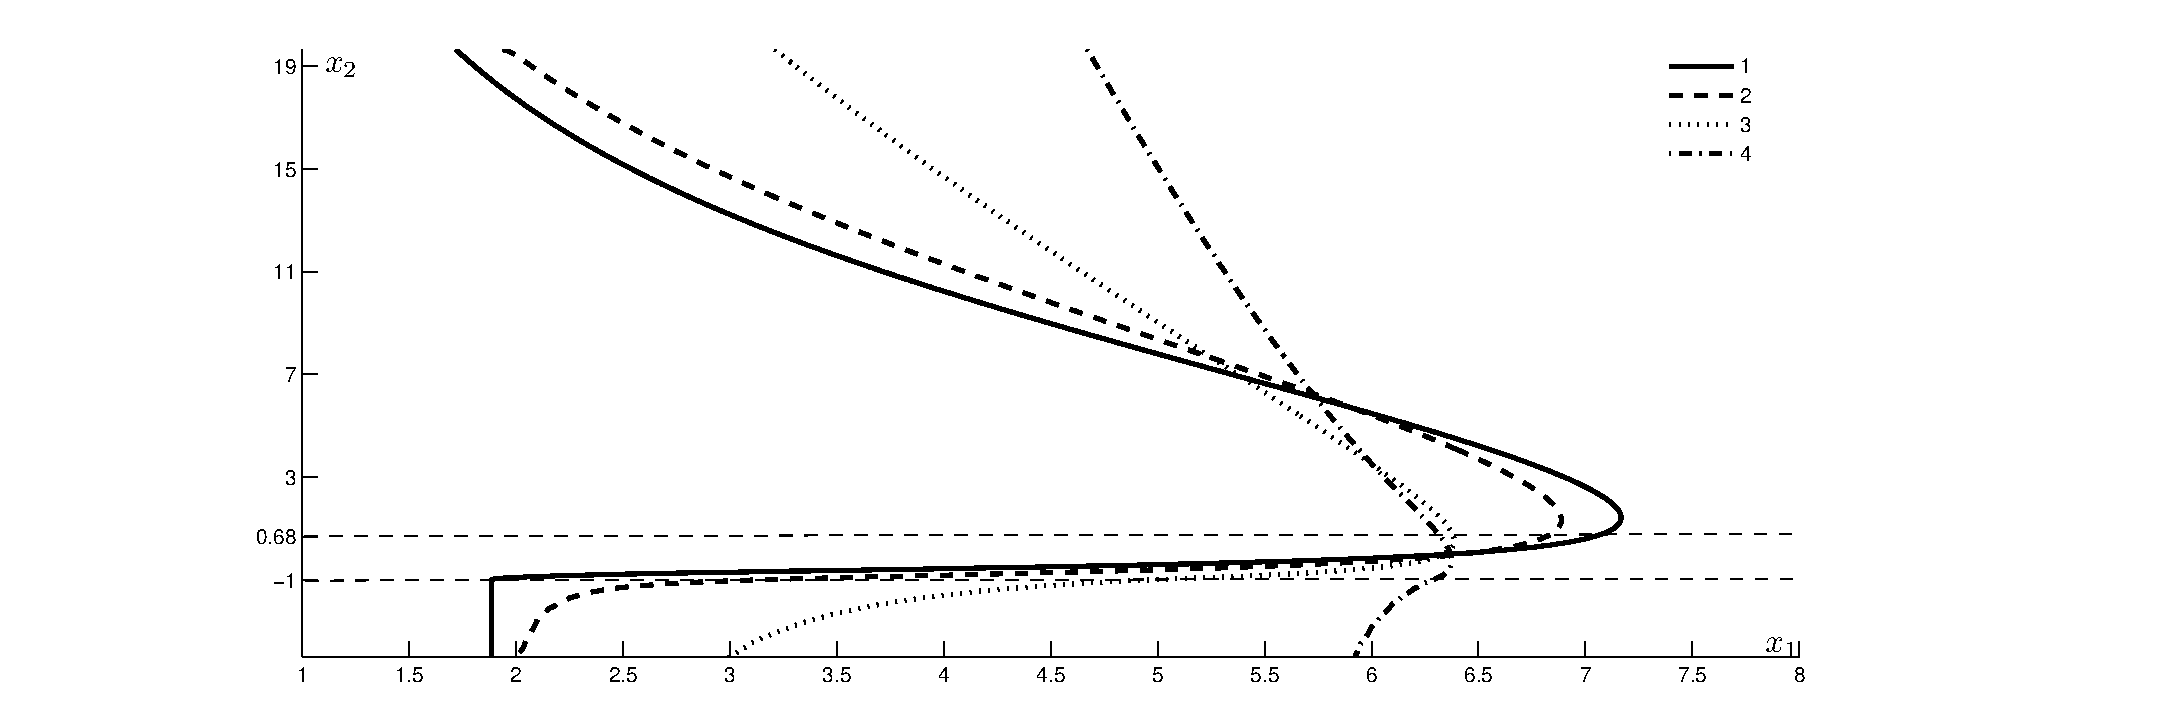
\includegraphics[width=1.1\textwidth]{images/C_1_f}
% \caption{График линии переключения $x^*(x_2)$ оптимальной стратегии $c^*$ выплаты дивидендов}
% \label{fig:1.2}
%\end{figure}
Кроме указанной барьерной структуры изчено также поведение $\theta^*$ --- оптимального объема капитала, инвестируемого в рисковый актив и $\alpha^*$ --- оптимального уровня перестрахования. Численных эксперименты указывают на ряд нетривиальных свойств оптимальных стратегий.

\textbf{В главе 2} рассматривается задача управления, в которой требуется как можно дольше удерживать стохастическую систему $X$ в заданной области $G$. Воздействие на систему $X$ требует расхода ресурса (или топлива). Задача состоит в том, чтобы использовать имеющееся количество ресурса оптимальным образом.
В отличие от подавляющего большинства известных работ, мы предполагаем что интенсивность потребления ресурса (топлива) ограничена.

Пусть $W=(W^1,\dots W^m)$ $m$-размерный винеровский процесс, в пространстве $(\Omega,\mathcal F,\mathsf P)$, где $\mathbb F=(\mathscr F_s)_{s\ge 0}$ --- минимальная пополненная естественная фильтрация процесса $W$ и управляемый процесс $X=(X^1,\dots,X^d)$ подчиняется системе стохастических дифференциальных уравнений
\begin{equation} \label{eq:2.1.1}
dX_t=b(X_t,\alpha_t) dt+\sigma(X_t,\alpha_t) dW_t, \quad X_0=x.
\end{equation}
$\mathbb F$-прогрессивно измеримый процесс $\alpha \in A=[\underline a, \overline a]$, $\underline a\le 0\le \overline a$ можно рассматривать как интенсивность потребления ресурса. Перерасход ресурса запрещен, то есть допустимы только управления $\alpha \in A$ для которых $Y_t \ge 0, t\ge 0$. Мы предполагаем что компоненты вектора сноса $b$ и матрицы диффузии $\sigma$ такие, что уравнение (\ref{eq:2.1.1}) имеет единственное $\mathbb F$-согласованное сильное решение на $[0,\infty)$.
Количество ресурса $Y$ удовлетворяет уравнению
\begin{equation} \label{eq:2.1.2}
dY_t=-|\alpha_t|dt,\quad Y_0=y.
\end{equation}

%Решение (\ref{eq:2.1.1}), (\ref{eq:2.1.2}) обозначим через $X^{x,y,\alpha}, Y^{x,y,\alpha}$.
%Процесс $\alpha$ назовем \emph{допустимым}, и будем использовать обозначение $\alpha \in \mathcal A(x,y)$, если $Y_t \ge 0$, $t\ge 0$. Допустимость означает, что перерасход ресурса запрещен.

Пусть $G\subset \mathbb R^d$ открытое множество, $0\in G$. Обозначим через
$\theta^{x,y,\alpha}=\inf\{t\ge 0:X_t^{x,y,\alpha}\not \in G\}$ время выхода процесса $X^{x,y,\alpha}$ из области $G$.
Целевой функционал $J$ и функцию Беллмана $v$ определены следующим образом:
\begin{equation} \label{eq:2.1.3}
J(x,y,\alpha)=\mathsf E\int_0^{\theta^{x,y,\alpha}} e^{-\beta t} f(X_t^{x,y,\alpha},\alpha_t)\,dt, \qquad
v(x,y)=\sup_{\alpha\in\mathcal A(x,y)} J(x,y,\alpha),
\end{equation}
где $\beta>0$, и $f:\mathbb R^d\times A\mapsto\mathbb R$ ограниченная непрерывная функция.

Рассмотрим семейство $\mathcal L^a$ ``инфинитезимальных генераторов'' диффузионного процесса $X$:
$$ \mathcal L^a\varphi(x)=b(x,a)\varphi_x(x)+ \frac{1}{2}\Tr(\sigma(x,a)\sigma^T(x,a)\varphi_{xx}(x)).$$
Здесь $\varphi_x=(\varphi_{x_i})_{i=1}^d$ --- градиент и $\varphi_{xx}=(\varphi_{x_i x_j})_{i,j=1}^d$ --- гессиан. Задача исследована при следующих предположениях. 
\begin{assumption} \label{as:2.1}
Существует решение $\psi\in C_b(\overline G)\cap C^2(G)$ задачи Дирихле
\begin{equation} \label{eq:2.2.5}
\beta\psi(x)-\widehat f(x)-\mathcal L^0\psi (x)=0, \ x\in G; \quad \psi=0 \ \textrm{ на }\ \partial G.
\end{equation}
\end{assumption}

\begin{assumption} \label{as:2.2}
Обозначим через $\overline v$ функцию Беллмана задачи с <<бесконечным топливом>>:
\begin{equation} \label{eq:2.2.11}
\overline v(x)=\sup_{\alpha\in\mathcal U} \mathsf E\int_0^{\theta^{x,\alpha}} e^{-\beta t} f(X_t^{x,\alpha},\alpha_t)\,dt,
\qquad \theta^{x,\alpha}=\inf\{t\ge 0: X_t^{x,\alpha}\not \in G\},
\end{equation}
где $X^{x,\alpha}$ --- решение (\ref{eq:2.1.1}). Краевая задача для соответствующего уравнения Гамильтона-Якоби-Беллмана
\begin{equation} \label{eq:2.2.12}
\beta \overline v- \sup_{a \in [\underline a, \overline a]} \left\{f(x,a)+ \mathcal L^a \overline v \right\}=0,\quad x\in G,
\end{equation}
\begin{equation} \label{eq:2.2.13}
\beta \overline v- \sup_{a \in [\underline a, \overline a]} \left\{f(x,a)+ \mathcal L^a \overline v \right\}=0 \quad
\textrm{или}\quad \overline v=0\quad \textrm{на }\ \partial G.
\end{equation}
удовлетворяет свойству сильной единственности.
\end{assumption}
\begin{assumption} \label{as:2.3}
Существует константа $K>0$ такая, что
$$ \sup_{x\in G}\left\{|f(x,a)-f(x,0)+\mathcal L^a\psi(x)-\mathcal L^0(x)\psi|\right\}\le K|a|.$$
\end{assumption}
В лемме \ref{lem:2.1} установлено, что задача (\ref{eq:2.1.1}) -- (\ref{eq:2.1.3}) сводится к задаче управления до момента выхода из области.
\begin{lemma} \label{lem:2.1}
Если выполняется условие \ref{as:2.1}, то функция Беллмана (\ref{eq:2.1.3}) допускает представление
\begin{equation} \label{eq:2.2.6}
v(x,y)=\sup_{\alpha\in\mathcal U}\mathsf E\left(\int_0^{T^{x,y,\alpha}} e^{-\beta t} f(X_t^{x,y,\alpha})\,dt+e^{-\beta T^{x,y,\alpha}}\psi(X_{T^{x,y,\alpha}}^{x,y,\alpha})\right),
\end{equation}
где $\mathcal U$ --- множество всех $\mathbb F$-прогрессивно измеримых стратегий $\alpha$ со значениями в $A$.
\end{lemma}

Для функции Беллмана $v$ доказана теорема единственности.
\begin{theorem} \label{th:2.1}
Пусть выполнены условия \ref{as:2.1}-\ref{as:2.3}. Тогда функция Беллмана $v$ является единственным ограниченным вязкостным решением уравнения
\begin{equation} \label{eq:2.2.4}
\beta v- \sup_{a \in [\underline a, \overline a]} \left\{f(x,a)+ \mathcal L^a v-|a|v_y \right\}=0,\quad (x,y)\in \Pi:=G\times (0,\infty),
\end{equation}
%$$H(x,v_x,v_y,v_{xx})=\sup_{a \in [\underline a, \overline a]} \left\{f(x,a)+ \mathcal L^a v-|a|v_y \right\},$$ 
непрерывным на $\overline\Pi$ и удовлетворяющим граничному условию
\begin{equation} \label{eq:2.2.15}
v=g\quad \textnormal{on\ } \partial\Pi.
\end{equation}
Здесь непрерывная функция $g$ на $\partial\Pi$ определена следующим образом
\begin{equation} \label{eq:2.2.14}
g(0,x)=\psi(x),\ \ x\in\overline G;\quad g(x,y)=0,\ x\in\partial G,\ y\ge 0.
\end{equation}
\end{theorem}

Для доказательства теоремы \ref{th:2.1} не удается
%Особенность уравнения (\ref{eq:2.2.4}) состоит в том, каким образом оно вырождается в граничных точках $(x,0)$. Данное вырождение не позволяет 
напрямую применить теорему сравнения \cite[теорема 2.1]{BarRou98}, \cite[теорема 2.1]{Cha04}. 
%Можно, однако, применить результаты \cite{MotSar08a} после некоторой подготовительной работы. 
Мы используем стохастический метод Перрона, разработанный в \cite{BaySir13}, и адаптированный к задаче управления до момента выхода из области в работе \cite{Rok14}. Этот метод работает с семействами $\mathcal V_-$, $\mathcal V_+$ стохастических суб- и суперрешений, которые порождают процессы суб- и супермартингального типа при суперпозиции с фазовым $X$ процессом, и оценивают функцию Беллмана снизу и сверху: $u\le v\le w$, $u\in\mathcal V_-$, $w\in\mathcal V_+$. Сущность стохастического метода Перрона состоит в том, что
$$ u_-(x)=:\sup_{u\in\mathcal V_-} u(x),\quad w_+(x):=\inf_{w\in\mathcal V_+} w(x)$$
являются соответственно вязкостным супер- и субрешениями уравнения HJB, и удовлетворяют граничному условию Дирихле в обобщенном вязкостном смысле: см. \cite[определение 7.4]{CraIshLio92} и \cite[теоремы 2, 3]{Rok14}. Если справедлив сильный принцип сравнения, обеспечивающий неравенство $u_-\ge w_+$ на $\Pi=G\times (0,\infty)$, то функция $u_-=v=w_+$ непрерывна на $\Pi$. Если, кроме того, $u_-\ge w_+$ on $\overline\Pi$, то $v$ непрерывна на $\overline\Pi$. Заметим, что основное предположение \cite{Rok14} состоит в справедливости сильного принципа сравнения, означающего, что для любых вязкостного субрешения $u$ и суперрешения $w$, удовлетворяющих граничному условию Дирихле в обобщенном вязкостном смысле, неравенство $u\le w$ спаведливо на $\Pi$. По-видимому, для рассматриваемой задачи такой результат неизвестен. Для преодоления этой трудности мы строим специальные стохастические суб- и суперрешения, совпадающие на определенных частях границы $\Pi$: см. лемму \ref{lem:2.2} (данная идея заимствована из \cite{BayZha15}). Этот прием позволяет заключить, что $u_-=v=w_+$ на $\partial\Pi$. Затем мы применяем стандартный принцип сравнения для вязкостных решений, удовлетворяющих граничному условию Дирихле в обычном смысле, и заключаем, что $v$ непрерывна на $\overline G\times [0,\infty)$. Таким образом получено короткое прямое доказательство теоремы \ref{th:2.1} без использования принципа динамического программирования.

Первая модель, иллюстрирующая теоретические результаты --- это задача оптимальной коррекции:
\begin{eqnarray*}
dX &=& -kXdt+\sigma dW_t-\alpha_t dt, \\
dY &=& -|\alpha_t|dt,
\end{eqnarray*}
где $\sigma>0$, $k$ --- некоторые константы и $\alpha_t\in [\underline a,\overline a]$, $-\underline a=\overline a>0$. Бесконечно малое приращение $dX$ системы может корректироваться с интенсивностью $\alpha$. Цель управления состоит в том, чтобы удерживать систему в интервале $G=(-l,l)$, $l>0$ как можно дольше. Случай $k>0$ (соотв., $k<0$) соответствует устойчивому (соотв., неустойчивому) равновесию $0$. 

По лемме \ref{lem:2.1} можно перейти к задаче управления до момента выхода:
$$ v(x,y)=\sup_{\alpha\in\mathcal U}\mathsf E\left(\int_0^{T^{x,y,\alpha}} e^{-\beta t}\,dt+e^{-\beta T^{x,y,\alpha}}\psi(X_{T^{x,y,\alpha}}^{x,y,\alpha})\right),$$
где $\psi$ --- решение задачи Дирихле для обыкновенного дифференциального уравнения:
\begin{eqnarray*}
&&\beta \psi -1 +kx\psi_x-\frac{1}{2}\sigma^2 \psi_{xx}=0, \quad x \in (-l,l)\\
&& \psi(-l)=\psi(l)=0.
\end{eqnarray*}
Ясно, что условия 1-3 выполняются. По теореме \ref{th:2.1} фунцкия $v$ является единственным ограниченным непрерывным вязкостным решением уравнения
\begin{equation} \label{eq:2.3.1}
\beta v -1-\frac{1}{2}\sigma^2 v_{xx}+\min_{a \in [\underline a,\overline{a}]}\{(kx+a)v_x+|a|v_y\}=0,\quad (x,y)\in (-l,l)\times(0,\infty),
\end{equation}
удовлетворяющим граничным условиям:
\begin{equation} \label{eq:2.3.2}
v(x,0)=\psi(x),\ x\in [-l,l];\quad v(-l,y)=v(l,y)=0,\ y>0.
\end{equation}

Для численного решения задачи использовались разностная схема и итерационный метод, аналогичные тем, которые применялись в первой главе. Расчеты показывают, что оптимальная стратегия имеет вид 
\begin{equation}
a^*(x,y) = \left \{
\begin{array}{cc} \overline a,& x< - h(y) \\
0,& |x|\le h(y),\\
\underline a, & x> - h(y),
\end{array}\right.
\end{equation} 
где $h$ --- монотонно убывающая положительная функция. Таким образом, область бездействия расширяется при уменьшении $y$. Это означает, что регулятор становится менее активным, когда количество ресурса $Y$ уменьшается. Более интересный и неожиданный эффект касается <<немонотонного>> поведения области бездействия по отношению к $k>0$. В неустойчивом случае $k<0$ область бездействия монотонно сжимается с ростом по $k$.


Вторая конкнетная модель, рассмотренная в главе 2, касается оптимального отслеживания стохастической системы. Предполагается, что имеется случайная цель $X^1$, которую должен отследить управляемый процесс $X^2$. Флуктуации $X^1$ описываются уравнением
\begin{eqnarray*}
dX^1_t &=& \mu(X^1_t) dt +\sigma dW_t,\quad \sigma>0,\\
\mu(x_1)&=& -k x_1 I_{\{|x_1|\le b\}} - k b I_{\{x_1\ge b\}}+k b I_{\{x_1\le -b\}},\quad b>0.
\end{eqnarray*}
Случай $k>0$ (соотв., $k<0$) соответствует устойчивой (соотв., неустойчивой) точке равновесия $0$ соответствующей детерминированной системы. Динамика следящего процесса $X^2$, управляемого <<расходом топлива>>, не подвержена воздействию шума:
$$ dX^2_t =\alpha_t dt,\quad dY_t =-|\alpha_t|dt,\quad \alpha_t\in [\underline a,\overline a].$$
Предполагается, что слежение прекращается, если цель <<потеряна из виду>>:
$$\tau=\inf\{t\ge 0:|X^1_t- X^2_t|\ge l\},\quad l>0.$$

Для целевого функционала (\ref{eq:2.1.4}) уравнение HJB (\ref{eq:2.2.4}) принимает вид
$$ \beta v-1-\mu(x_1)v_{x_1}-\frac{1}{2}\sigma^2 v_{x_1 x_1}+\min_{a\in [\underline a,\overline a]}\{|a| v_y-a v_{x_2}\}=0,\quad
(x,y)\in G\times (0,\infty), $$
где $G=\{x:|x_1-x_2|<l\}$. Граничные условия (\ref{eq:2.2.15}) преобразуются к следующей форме
$$ v=0\quad \textrm{на } \partial G\times [0,\infty);\quad v=\psi\quad \textrm{на } G\times\{0\},$$
где $\psi$ --- решение краевой задачи
\begin{eqnarray}
&&\beta \psi-1-\mu(x_1)\psi_{x_1}-\frac{1}{2}\sigma^2 \psi_{x_1 x_1}=0,\quad x_1\in (x_2-l,x_2+l),\label{eq:2.4.1}\\
&&\psi(x_2-l,x_2)=\psi(x_2+l,x_2)=0.\label{eq:2.4.2}
\end{eqnarray}

Проведены расчеты оптимальных стратегий отслеживания в устойчивом и неустойчивом случаях в переменных
$$z_1=(x_1+x_2)/\sqrt 2,\quad z_2=(x_1-x_2)/\sqrt 2,$$
полученных преобразованием поворота. Фактически, данные стратегии также характеризуются областями бездействия. 

\textbf{В третьей главе} рассматриваются оптимальные стратегии производства и назначения цен в динамической модели фирмы-монополиста.
Предположим, что фирма может производить некоторый товар с интенсивностью $\alpha_t\in A$, где $A$ --- замкнутое подмножество $\mathbb R_+=[0,\infty)$. Будучи монополистом, фирма может устанавливать цену $p_t\ge 0$ за единицу товара.
Предполагая, что интенсивность спроса является известной строго убывающей функцией цены: $q=D(p)$. Удобно считать, что фирма динамически выбирает интенсивность спроса $q_t\in Q$. Множество $Q\subset\mathbb R_+$ предполагается компактным. Уровень товарного запаса $X$ удовлетворяет уравнению
\begin{equation} \label{eq:3.2.1}
X_t=x+\int_0^t (\alpha_s-q_s)\,ds,\quad t\ge 0.
\end{equation}
Пусть отложенный спрос недопустим: $X_t\ge 0$, и множества $Q$, $A$ удовлетворяют следующим условиям:
\begin{equation} \label{eq:3.2.2}
0\in A\cap Q,\quad A\backslash\{0\}\neq\emptyset,\quad Q\backslash\{0\}\neq\emptyset.
\end{equation}
Решение уравнения (\ref{eq:3.2.1}) также будем обозначать через $X^{x,\alpha,q}$.

Пусть $R(q)=qp=qD^{-1}(q)$ --- функция мгновенного дохода, и $C(\alpha)$ --- функция мгновенных затрат. Цель фирмы состоит в том, чтобы максимизировать дисконтированную прибыль на бесконечном горизонте:
$$ \int_0^\infty e^{-\beta t} (R(q_t)-C(\alpha_t))\,dt,\quad \beta>0.$$

Предполагается, что $R:Q\mapsto\mathbb R_+$ непрерывна, $R(0)=0$, и $C:A\mapsto\mathbb R_+$ --- неубывающая непрерывная функция. Если множество $A$ является неограниченным, то мы дополнительно предполагаем, что $C$ --- $1$-коэрцитивная функция:
\begin{equation} \label{eq:3.2.3}
C(\alpha)/\alpha\to +\infty,\quad A\ni\alpha\to+\infty.
\end{equation}

Обозначим через $\mathscr A(x)$ множество всех борелевских функций $\alpha:\mathbb R_+\to A$, $q:\mathbb R_+\to Q$ таких, что уровень товарного запаса (\ref{eq:3.2.1}) неотрицателен. Функция Беллмана $v$ определяется следующим образом
\begin{equation} \label{eq:3.2.4}
v(x)=\sup_{(\alpha,q)\in\mathscr A(x)}\int_0^\infty e^{-\beta t} (R(q_t)-C(\alpha_t))\,dt, \quad x\ge 0.
\end{equation}
Введем гамильтониан
\begin{equation} \label{eq:3.2.5}
H(z)=\widehat R(z)+\widehat C(z),\quad \widehat R(z)=\sup_{q\in Q}\{R(q)-qz\},\quad
\widehat C(z)=\sup_{\alpha\in A}\{\alpha z-C(\alpha)\}.
\end{equation}
\begin{lemma} \label{lem:3.1}
Предположим, что множество $A$ компактно. Тогда функция Беллмана $v$ ограничена и равномерной непрерывна. Кроме того, $v$ является единственным вязкостным решением с ограничениями (constrained viscosity solution: CVS) уравнения 
\begin{equation} \label{eq:3.2.6}
\beta u(x)-H(u'(x))=0,\quad x\ge 0,
\end{equation}
в классе ограниченных равномерно непрерывных функций.
\end{lemma}
Результаты, собранные в этой лемме, доказаны в \cite{Son86} (теоремы 3.3, 2.1, 2.2).
Заметим, что предположение (A3) работы \cite{Son86}, касающееся существования <<внутреннего направления>>, выполняется, так как $\sup\{\alpha-q:\alpha\in A, q\in Q\}>0$ в силу (\ref{eq:3.2.2}).

Обозначим через $\mathscr M_H=\arg\min_{z\in\mathbb R} H(z)$ множество точек минимума $H$, а через $\zeta=\min\mathscr M_H\ge 0$ наименьшую точку минимума функции $H$.
\begin{theorem} \label{th:3.1}
Функция Беллмана $v$ ограничена:
$$ v(x)\le \frac{H(0)}{\beta}=\lim_{y\to\infty} v(y)$$
и допускает следующее представление:
\begin{itemize}
\item[(i)] если $\zeta=0$, то
\begin{equation} \label{eq:3.2.9}
v(x)=H(0)/\beta,
\end{equation}
\item[(ii)] если $\zeta>0$ то
\begin{equation} \label{eq:3.2.10}
v(x)=\frac{H(\xi(x))}{\beta}=\frac{H(\zeta)}{\beta}+\int_0^x\xi(y)\,dy,
\end{equation}
где $\xi(x)$ определяется уравнением
$$x=\Psi(\xi):=-\int_\xi^{\zeta}\frac{H'(z)}{\beta z}\,dz,\quad \xi\in (0,\zeta],\quad x\ge 0.$$
\end{itemize}
В случае (ii) $v$ является строго возрастающей и строго вогнутой. Кроме того, $v'$ абсолютно непрерывна и удовлетворяет условиям $v'(0)=\zeta$, $\lim_{x\to\infty} v'(x)=0.$ Наконец, $v''<0$ п.в.
\end{theorem}

В ходе доказательства теоремы \ref{th:3.1} было установлено что, переход от множества $A$ к $A\cap [0,c]$ не влияет на функцию Беллмана $v$ при достаточно больших $c$.

Заметим также, что если $\zeta>0$, то оптимальная дисконтированная прибыль не превосходит $H(0)/\beta$. Если $\zeta=0$, то дисконтированная прибыль $H(0)/\beta$ может быть получена при нулевом начальном запасе. Более того, при этом любой начальный запас $x>0$ бесполезен.

Введем понятие \emph{овыпукленной задачи}:
\begin{equation} \label{eq:3.2.17}
\widetilde v(x)=\sup_{(\alpha,q)\in\widetilde{\mathscr A}(x)}\int_0^\infty e^{-\beta t}(\widetilde R(q_t)-\widetilde C(\alpha_t))\,dt,
\end{equation}
где $\widetilde{\mathscr A}(x)$ --- множество измеримых по Борелю функций $\alpha:\mathbb R_+\mapsto\co A$, $q:\mathbb R_+\mapsto \co Q$ таких, что $X_t^{x,\alpha,q}\ge 0$. Заметим, что $\widetilde C$ по-прежнему удовлетворяет условию (\ref{eq:3.2.3}): см. \cite[глава E, предложение 1.3.9(ii)]{HirUrrLem01}.

Введем также ослабленную задачу. Для этого расширим класс стратегий производства и назначения цены. \emph{Распределенные управления} $q_t(dy)$ и $\alpha_t(dy)$ представляют собой отображения отрезка $[0,\infty)$ в множества вероятностных мер на $Q$ и $A$ такие, что функции
$$ t\mapsto\int_Q\varphi(y)\,q_t(dy),\qquad t\mapsto\int_A\varphi(y)\,\alpha_t(dy)$$
измеримы по Борелю для любой непрерывной функции $\varphi$. Динамика движения товарного запаса при использовании распределенных управлений определяется следующим образом
$$ X_t=x+\int_0^t\int_Q y\,q_s(dy)ds-\int_0^t\int_A y\,\alpha_s(dy)ds.$$
Класс $\mathscr A_r(x)$ допустимых распределенных стратегий содержит лишь те, которые удерживают $X_t$ в неотрицательной области. Соответствующая функция Беллмана определяется следующим образом:
\begin{equation} \label{eq:3.2.18}
v_r(x)=\sup_{(\alpha,q)\in\mathscr A_r(x)}\left(\int_0^\infty e^{-\beta t}\int_Q R(y)\,q_t(dy)dt -\int_0^\infty e^{-\beta t} \int_A C(y)\,\alpha_t(dy)dt\right).
\end{equation}
Задачу (\ref{eq:3.2.18}) будем называть \emph{ослабленной}.

\begin{theorem} \label{th:3.2}
Функции Беллмана (\ref{eq:3.2.4}), (\ref{eq:3.2.17}), (\ref{eq:3.2.18}) соответствующие исходной, овыпукленной и ослабленной задачам совпадают:
$v=v_r=\widetilde v.$
\end{theorem}

Равенство $v=v_r$ для задачи с фазовыми ограничениями в случае компактных множеств состояний и управлений было установлено в \cite{Lor87}.

Далее, в главе 3 рассматривается случай нулевого начального запаса: $X_0=0$. Для любой константы $\widehat u\in Q\cap A$ \emph{статическая стратегия} $\alpha_t=q_t= \widehat u$ допустима. Если она оптимальна, то
\begin{equation} \label{eq:3.3.1}
\widehat u\in\mathscr M:=\arg\max_{u\in Q\cap A}\{R(u)-C(u)\}.
\end{equation}
Для $\eta\in\mathbb R$ положим
$$\mathscr M_R(\eta)=\arg\max_{q\in Q}\{R(q)-\eta q\},\qquad
\mathscr M_C(\eta)=\arg\max_{\alpha\in A}\{\alpha\eta-C(\alpha)\},$$
и $\mathscr M_\eta=\mathscr M_R(\eta)\cap\mathscr M_C(\eta)$.
%В разделе доказываются следующие теоремы:
\begin{theorem} \label{th:3.3}
Следующие условия эквивалентны.
\begin{itemize}
\item[(i)] Статическая стратегия $\alpha_t=q_t= \widehat u\in\mathscr M$ является оптимальной.
\item[(ii)] $\mathscr M_\eta\neq\emptyset$ для некоторого $\eta\in\mathbb R$.
\item[(iii)] $\mathscr M_\zeta\neq\emptyset$.
\end{itemize}
%Assume that $R\not\equiv 0$ and $C$ is strictly increasing. If a stationary strategy is not optimal, then there is no optimal strategy.
Если $\mathscr M_\eta\neq\emptyset$, то $\eta$ является точкой минимума функции $H$ и $\mathscr M_\eta=\mathscr M$.
\end{theorem}

Чтобы дать экономическую интерпретацию условия $\mathscr M_\eta\neq\emptyset$, предположим что в некоторой фирме управление производственным цехом и отделом продаж происходит независимо друг от друга. Производственный цех продает товар отделу продаж по некоторой \emph{теневой} цене $\eta$ и получает мгновенный доход $\eta\alpha-C(\alpha)$. Отдел продаж получает мгновенный доход $R(q)-\eta q$ продавая товар на рынке. Для каждой возможной цены $\eta$ отделы пытаются выбрать оптимальные стратегии $\widehat\alpha$, $\widehat q$. Равновесие $\widehat\alpha=\widehat q$ соответствует теневой цене $\eta$ такой, что $\mathscr M_\eta\neq\emptyset$. По теореме \ref{th:3.2} статическая стратегия является оптимальной в точности тогда, когда данное равновесие существует.

Аналогично равновесию механической системы, равновесная теневая цена $\eta$ может быть определена как точка минимума гамильтониана $H$. По теореме \ref{th:3.1} наименьшая теневая цена $\zeta$ совпадает с предельной непрямой полезностью $v'(0)$ нулевого запаса.

\begin{theorem} \label{th:3.4}
Предположим что множества $Q$, $A$ выпуклы, функция $R$ вогнута и функция $C$ выпукла.
Тогда для любого $\eta\in\mathscr M_H$ имеем
$\mathscr M_\eta\neq\emptyset$.
Следовательно, стационарная стратегия является оптимальной.
\end{theorem}
По теоремам \ref{th:3.3}, \ref{th:3.4} для овыпукленной задачи (\ref{eq:3.2.17}) стационарная стратегия $\widetilde\alpha_t=\widetilde q_t=\widetilde u$,
\begin{equation} \label{eq:3.3.8}
\widetilde u\in\arg\max\{\widetilde R(u)-\widetilde C(u):u\in\co Q\cap\co A\},
\end{equation}
оптимальна для нулевого начального запаса, и
$$\widetilde v(0)=\frac{\widetilde R(\widetilde u)-\widetilde C(\widetilde u)}{\beta}.$$
Далее, cуществуют $\gamma\in (0,1)$, $\nu\in (0,1)$, $q^i\in Q$, $\alpha^i\in A$, $i=1,2$ такие, что
\begin{equation} \label{eq:3.3.9}
\widetilde u=\gamma q^1+(1-\gamma) q^2=\nu\alpha^1+(1-\nu)\alpha^2,
\end{equation}
\begin{equation} \label{eq:3.3.10}
\widetilde R(\widetilde u)=\gamma R(q^1)+(1-\gamma) R(q^2),\quad \widetilde C(\widetilde u)=\nu C(\alpha^1)+(1-\nu) C(\alpha^2).
\end{equation}
Установлено, что распределенные управления
\begin{equation} \label{eq:3.3.11}
\overline q_t(dx)=\gamma\delta_{q^1}(dx)+(1-\gamma)\delta_{q^2}(dx),\quad
\overline \alpha_t(dx)=\nu\delta_{\alpha^1}(dx)+(1-\nu)\delta_{\alpha^2}(dx),
\end{equation}
где $\delta_a$ --- мера Дирака, сконцентрированная в точке $a$, являются оптимальными для задачи (\ref{eq:3.2.18}) при нулевом начальном запасе.

Для случая положительного начального запаса доказана следующая теорема:
\begin{theorem} \label{th:3.6}
Пусть $F\subset (0,\zeta)$ --- ко-счетное множество, где выпуклые функции $\widehat R$, $\widehat C$ дифференцируемы. Положим
$$ \{\widehat q(z)\}=\arg\max_{q\in \co Q} \{\widetilde R(q)-q z\},\quad
\{\widehat\alpha(z)\}=\arg\max_{\alpha\in\co A}\{\alpha z-\widetilde C(\alpha)\},\quad z\in F,$$
$$\widehat u\in\arg\max(\widetilde R(u)-\widetilde C(u):u\in\co Q\cap\co A).$$
Для заданного начального запаса $x>0$ положим
$$\tau=\frac{1}{\beta}\ln\frac{v'(0)}{v'(x)}$$
и определим $X$ с помощью уравнения
\begin{equation} \label{eq:3.4.3}
v'(X_t)=v'(x)e^{\beta t},\quad t\in [0,\tau].
\end{equation}

Далее, положим $\mathscr T=\{t\in [0,\tau]:v'(X_t)\in F\}$ и рассмотрим стратегию
\begin{equation} \label{eq:3.4.4}
\alpha^*_t=\widehat\alpha(v'(X_t)),\quad q^*_t=\widehat q(v'(X_t)),\quad t\in\mathscr T,
\end{equation}
\begin{equation} \label{eq:3.4.5}
\alpha^*_t=q^*_t=\widehat u,\quad t>\tau.
\end{equation}
На счетном множестве $[0,\tau]\backslash \mathscr T$ значения $\alpha^*_t$, $q_t^*$ могут быть определены произвольным образом.

(i) Стратегия (\ref{eq:3.4.4}) является оптимальной для овыпукленной задачи (\ref{eq:3.2.17}).

(ii) Имеем
\begin{equation} \label{eq:3.4.6}
(\alpha_t^*,q_t^*)\in\dom C\times\dom R,\quad \widetilde C(\alpha^*_t)=C(\alpha^*_t),\quad \widetilde R(\alpha_t^*)=R(\alpha_t^*),\quad t\in\mathscr T.
\end{equation}

(iii) Существуют $q^i\in Q$, $\alpha^i\in A$, $i=1,2$ и $\gamma\in (0,1)$, $\nu\in (0,1)$ такие, что справедливы равенства (\ref{eq:3.3.9}), (\ref{eq:3.3.10}). Заменяя (\ref{eq:3.4.5}) статическим распределенным управлением
\begin{equation} \label{eq:3.4.7}
\overline q(dx)=\gamma\delta_{q^1}(dx)+(1-\gamma)\delta_{q^2}(dx),\quad
\overline \alpha(dx)=\nu\delta_{\alpha^1}(dx)+(1-\nu)\delta_{\alpha^2}(dx),
\end{equation}
получаем решение ослабленной задачи (\ref{eq:3.2.18}).

(iv) Если $\mathscr M_\zeta\neq\emptyset$, то заменяя (\ref{eq:3.4.5}) на
\begin{equation} \label{eq:3.4.8}
\widehat u\in\arg\max_{u\in Q\cap A}(R(u)-C(u)),
\end{equation}
получаем оптимальное решение задачи (\ref{eq:3.2.4}).
\end{theorem}

В заключительной части главы 3 рассматривается пример Арвана-Мозеса, где спрос является линейным, а получаемый мгновенный доход выглядит следующим образом:
$$ R(q)=(A-Bq)q,\quad q\in [0,A/B].$$
Функция затрат
$$ C(\alpha)=\alpha^3/3-K\alpha^2+K^2\alpha,\quad \alpha\ge 0$$
выпукла на $[0,K]$ и вогнута на $[K,\infty)$. Здесь предполагается что $A, B, K>0$.
Заметим, что функция $C$ является строго возрастающей и $1$-коэрцитивной. Функция $R$ строго вогнута.

Оптимальная статическая стратегия для нулевого начального запаса 
$$ \widehat u\in\arg\min_{u\in [0,A/B]}(R(u)-\widetilde C(u))$$
имеет вид
\begin{equation} \label{eq:3.6.1}
\widehat u=\begin{cases}
0,& A\le K^2/4,\\
(A-K^2/4)/(2B),& K^2/4\le A\le 3BK+K^2/4,\\
-B+K+\sqrt{B^2-2BK+A},& A\ge 3BK+K^2/4.
\end{cases}
\end{equation}

Для $A\le K^2/4$ и $A\ge 3BK+K^2/4$ имеем $\widetilde C(\widehat u)=C(\widehat u)$. Следовательно, в этих случаях $\alpha_t=q_t=\widehat u$ является оптимальным решением исходной задачи (\ref{eq:3.3.4}). Если
\begin{equation} \label{eq:3.6.2}
\frac{K^2}{4}< A< 3BK+\frac{K^2}{4},
\end{equation}
то $\widehat u$ принадлежит интервалу $(0,3K/2)$, где $\widetilde C$ линейна и $\widetilde C<C$. В этом случае оптимальная распределенная стратегия производства определяется формулами (\ref{eq:3.3.9}) -- (\ref{eq:3.3.11}):
\begin{equation} \label{eq:3.6.3}
\overline\alpha_t(dx)=\nu\delta_0+(1-\nu)\delta_{3K/2},\quad (1-\nu)\frac{3K}{2}=\widehat u=\left(A-\frac{K^2}{4}\right)\frac{1}{2B}.
\end{equation}

Таким образом, для нулевого начального запаса обычная статическая стратегия не является оптимальной, если и только если выполнено условие (\ref{eq:3.6.2}). 
%В этом случае вместо распределенной стратегии (\ref{eq:3.6.3}) можно использовать приближенно оптимальную стратегию (\ref{eq:3.3.15}), (\ref{eq:3.3.16}). При использовании этой стратегии запас остается близким к $0$: $X_t\le b\varepsilon$, $b>0$, и демонстрирует циклическое поведение накопления-сокращения, описанное в \cite{ArvMos81}. Однако, оно может не производить дисконтированную прибыль близкую к оптимальной, если циклы накопления-сокращения не малы.
Для произвольного начального запаса оптимальная стратегия определяется следующим образом.

(i) Если $A\le K^2/4$, то фирма должна оптимально продать начальный запас:
$$ \dot X_t=-\widehat q(v'(X_t))=-\frac{A-v'(X_t)}{2B}<0,\quad X_t>0.$$
Производство отсутствует.

(ii) Если $\quad K^2/4<A< K^2/4+3BK$, то производство начинается после продажи начального запаса, и распределенная производственная стратегия (\ref{eq:3.6.3}) должна соответствовать спросу $\widehat q(\zeta)=\widehat u=(A-K^2/4)/2B$.

(iii) Если $A\ge K^2/4+3BK$, то производство начинается после того, как уровень товарного запаса падает ниже $\widehat x$: $v'(\widehat x)=K^2/4$. При этом товарный запас продолжает уменьшаться до $0$ и стабилизируется на этом уровне. Оптимальные спрос и интенсивность производства соответствующего устойчивого режима равны значению $\widehat u$, определенному в (\ref{eq:3.6.1}).


\textbf{В главе 4} исследуется одна из версий задачи позиционирования объекта, находящегося под воздействием случайных факторов.
Рассмотрим некоторый случайный процесс $S$, согласованный с естественной фильтрацией $\mathbb F=(\mathscr F_s)_{s\in [0,T]}$ винеровского процесса $W$. Будем считать, что положение объекта в терминальный момент времени $T$ имеет вид
$$X_T = X_0+\gamma_0(S_\tau-S_0) +\gamma_\tau(S_T-S_\tau),$$
%Здесь $X_0, \gamma_0$ --- начальные положение и интенсивность воздействия, а стратегия изменения интенсивности воздействия представлена парой $(\gamma_\tau,\tau)$, 
где $\tau$ момент остановки относительно $\mathbb F$, а $\gamma_\tau $ --- $\mathscr F_\tau$ - измеримая случайная величина. Основной пример: $S$ --- цена рискового актива, $\gamma_0, \gamma_\tau$ --- портфель, $X$ --- капитал. Цель состоит в минимизации среднеквадратического отклонения $X_T$ от заданного фиксированного уровня $H$:
\begin{equation}
\label{eq:4.1.1}
\mathsf E[(X_T-H)^2] \to \min_{(\gamma_\tau,\tau)},
\end{equation}
что может рассматриваться, как хеджирование в среднеквадратическом за счет однократного изменения портфеля в выбранный момент времени $\tau$.

Данная задача сводится к задаче оптимальной остановки:
\begin{equation}
\label{eq:4.1.4}
\mathsf E\left[(\widehat H - \gamma_0 S_\tau)^2 \left( 1-\frac{\mathsf E((S_T-S_\tau) | \mathscr F_\tau)^2}{\mathsf E((S_T-S_\tau)^2 | \mathscr F_\tau)}\right)\right] \to \min_{\tau},
\end{equation}
где $\widehat H = H-X_0+\gamma_0 S_0$.

Для моделей броуновского движения со сносом и геометрического броуновского движения: $$dS_t=\mu dt+\sigma dW_t, \quad dS_t=\mu S_t dt+\sigma S_t dW_t$$
положим
$$
\phi_1(t)=\frac{\sigma^2}{\mu^2(T-t)+\sigma^2}, \quad \phi_2(t)=\frac{e^{2\mu(T-t)}(e^{\sigma^2(T-t)}-1)}{e^{(2\mu+\sigma^2)(T-t)}-2e^{\mu(T-t)}+1}
$$ 
соответственно. Задача (\ref{eq:4.1.4}) принимает вид
\begin{equation}
\label{eq:4.1.7}
\mathsf E[h(S_\tau)\phi_i(\tau)] \to \min_{\tau},
\end{equation} 
где $h(S_t)=(\widehat H - \gamma_0 S_t)^2$, и

Для оценки оптимального момента остановки была использована интегральная форма задачи (\ref{eq:4.1.7}):
\begin{equation}
\label{eq:4.2.1}
h(S_0)\phi_i(0)+\mathsf E\left [\int_0^\tau F(t,S_t)dt \right ] \to \min_{\tau},
\end{equation}
где $F(t,s)=h(s)\phi_i'(t)+ h'(s)\phi_i(t)\mu(s)+\frac{1}{2}h''(s)\phi_i(t)\sigma^2(s).$ Было установлено что оптимальный момент остановки $\hat \tau$ удовлетворяет оценке $\hat \tau \ge \tau^*$, где 
\begin{equation} \label{eq:4.2.2}
\tau^*=\inf_t\{t\ge 0: F(t,S_t) \ge 0\} \wedge T.
\end{equation}
Отметим, что если $\mu=0$, то $\tau^*=0$ и $\gamma^*_\tau=0$. При $\mu \neq 0$ область продолжения, определяющая момент $\tau^*$, имеет вид
\begin{align*}
&\{(t,s): F(t,s) \le 0\}=\{(t,s): s_1(t) \le s \le s_2(t)\},\\
s_{1,2}(t)&=\frac{\widehat H}{\gamma_0}-\frac{\sigma^2}{\mu}-\mu(T-t) \pm \sqrt{\mu^2(T-t)^2+\sigma^2(T-t)},\\
s_{1,2}(t)&=\frac{H}{\gamma_0}\frac{\mu\phi_2(t)+\phi_2^\prime(t)\pm \sqrt{\mu^2\phi_2^2(t)-\sigma^2\phi_2(t)\phi_2^\prime(t)}}{(\sigma^2+2\mu)\phi_2(t)+\phi_2^\prime(t)}
\end{align*}
в случае броуновского движения со сносом и геометрического броуновского движения соответственно. 

Для численного решения задачи использовалось уравнение Гамильтона-Якоби-Беллмана
\begin{align}
\label{eq:4.3.2}
&\min{\left\{v_t - [\mu(x)v_{s}+\frac{1}{2}\sigma^2(s) v_{ss}],h(s)\phi_i(t)-v\right\}}=0,\ \ (t,s)\in G,\\
&v(T,s)=h(s)\phi_i(T)
\end{align}
для задачи (\ref {eq:4.1.7}).
Для модели броуновского движения со сносом $G=[0,T] \times\mathbb R$, $\mu, \sigma$ являются константами.
В модели геометрического броуновского движения $G=[0,T] \times [0,+\infty)$, $\mu(s)=\mu s, \sigma(s)=\sigma s$.

Для проведения расчетов в главе 4 использована разностная схема, обладающая свойствами аппроксимации, монотонности и устойчивости. Данная схема является сходящейся, так как для задачи (\ref{eq:4.3.2}) справедлива теорема сравнения. Проведено сравнение рассчитанных областей остановки с оценками, которые определяются формулой (\ref{eq:4.2.2}).

